\documentclass[tikz,border=8pt]{standalone}
\usepackage{amsmath,amssymb}
\usetikzlibrary{arrows.meta,automata,positioning,quotes}
\begin{document}
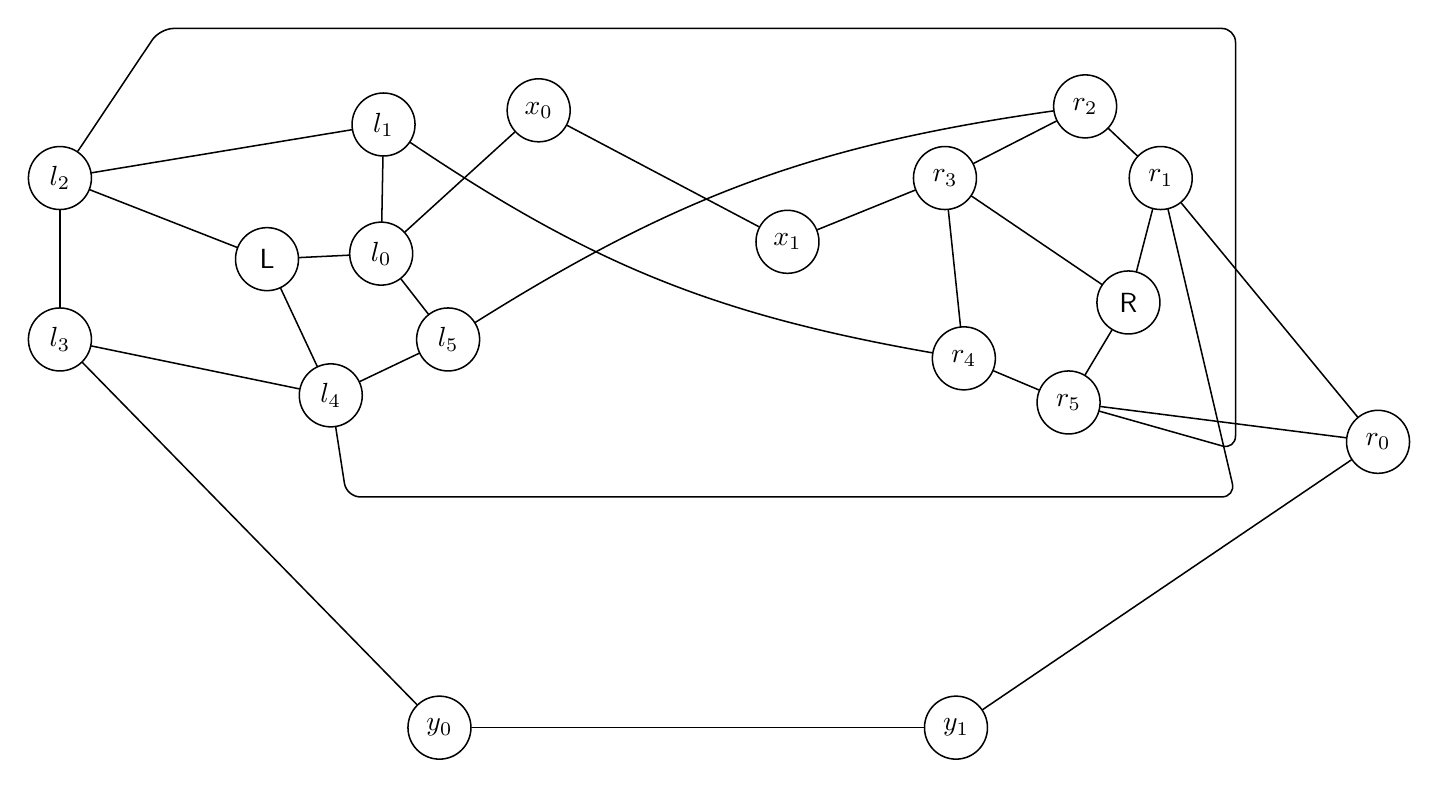
\begin{tikzpicture}[x=1cm,y=1cm]
\tikzset{
  graphnode/.style={circle,draw=black,line width=0.55pt,minimum size=8mm,inner sep=1pt,font=\sffamily},
  graphedge/.style={draw=black,line width=0.55pt,line cap=round,line join=round},
  directed/.style={graphedge,-{Stealth[length=2.4mm,width=2.0mm]}},
  undirected/.style={graphedge}
}
\node[graphnode] (n_L) at (-5.45,0.15) {L};
\node[graphnode] (n_l0) at (-4.00,0.22) {$l_{0}$};
\node[graphnode] (n_l1) at (-3.97,1.86) {$l_{1}$};
\node[graphnode] (n_l2) at (-8.08,1.18) {$l_{2}$};
\node[graphnode] (n_l3) at (-8.08,-0.87) {$l_{3}$};
\node[graphnode] (n_l4) at (-4.64,-1.58) {$l_{4}$};
\node[graphnode] (n_l5) at (-3.15,-0.87) {$l_{5}$};
\node[graphnode] (n_R) at (5.49,-0.40) {R};
\node[graphnode] (n_r0) at (8.66,-2.17) {$r_{0}$};
\node[graphnode] (n_r1) at (5.90,1.18) {$r_{1}$};
\node[graphnode] (n_r2) at (4.94,2.09) {$r_{2}$};
\node[graphnode] (n_r3) at (3.16,1.18) {$r_{3}$};
\node[graphnode] (n_r4) at (3.40,-1.11) {$r_{4}$};
\node[graphnode] (n_r5) at (4.73,-1.67) {$r_{5}$};
\node[graphnode] (n_x0) at (-2.00,2.04) {$x_{0}$};
\node[graphnode] (n_x1) at (1.16,0.37) {$x_{1}$};
\node[graphnode] (n_y0) at (-3.26,-5.80) {$y_{0}$};
\node[graphnode] (n_y1) at (3.30,-5.80) {$y_{1}$};
\draw[undirected] (n_l0) -- (n_l1);
\draw[undirected] (n_l1) -- (n_l2);
\draw[undirected] (n_l2) -- (n_l3);
\draw[undirected] (n_l3) -- (n_l4);
\draw[undirected] (n_l4) -- (n_l5);
\draw[undirected] (n_l5) -- (n_l0);
\draw[undirected] (n_L) -- (n_l0);
\draw[undirected] (n_L) -- (n_l2);
\draw[undirected] (n_L) -- (n_l4);
\draw[undirected] (n_r0) -- (n_r1);
\draw[undirected] (n_r1) -- (n_r2);
\draw[undirected] (n_r2) -- (n_r3);
\draw[undirected] (n_r3) -- (n_r4);
\draw[undirected] (n_r4) -- (n_r5);
\draw[undirected] (n_r5) -- (n_r0);
\draw[undirected] (n_R) -- (n_r1);
\draw[undirected] (n_R) -- (n_r3);
\draw[undirected] (n_R) -- (n_r5);
\draw[undirected] (n_l0) -- (n_x0);
\draw[undirected] (n_x0) -- (n_x1);
\draw[undirected] (n_x1) -- (n_r3);
\draw[undirected] (n_l3) -- (n_y0);
\draw[undirected] (n_y0) -- (n_y1);
\draw[undirected] (n_y1) -- (n_r0);
\draw[undirected] (n_l1) to[bend right=12] (n_r4);
\draw[undirected,rounded corners=5pt] (n_l2) -- (-6.81,3.08) -- (6.85,3.08) -- (6.85,-2.27) -- (n_r5);
\draw[undirected,rounded corners=5pt] (n_l4) -- (-4.44,-2.87) -- (6.85,-2.87) -- (n_r1);
\draw[undirected] (n_l5) to[bend left=12] (n_r2);
\end{tikzpicture}
\end{document}
